\chapter{Etat de l'art}
\paragraph*{} A rédiger
\section{Différents niveaux de chiffrements}
\paragraph*{} A rédiger
\section{Chiffrement de disque sur Linux et FreeBSD}
\paragraph*{} A rédiger
\subsection{Organisation dans le système d'exploitation}
\paragraph{}
Dans le cas de Linux, le chiffrement de disque est géré par le module noyau
{\em dm-crypt}, qui est un module qui dépend du module plus général
{\em device-mapper} qui gère les transformations de disque sous linux (RAID, 
LVM, Cache, ...). Le module dm-crypt gère la table appelée {\em crypt table}
qui permet d'associer un device à un chiffrement notamment. La table permet
la lecture des données sur le disque. A celà s'ajoute le programme cryptsetup
qui permet de lire des métadonnées stockées sur le disque pour remplir la {\em
crypt table}. Le programme s'occupe notamment du déchiffrement de la clé, de 
la lecture et de l'écriture des métadonnées sur le disque. L'organisation est 
donc la suivante :

\paragraph{}
\begin{figure}[h]
\centering
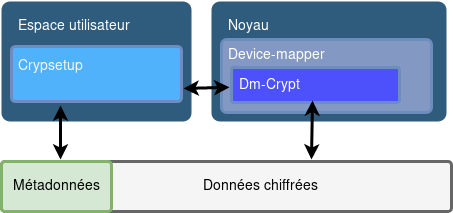
\includegraphics[width=.8\linewidth]{etat_art/organisation_linux.png}
\caption{\label{fig:OrgLinux}Organisation du code dans Linux}
\end{figure}

\paragraph{}
L'organisation reflétée par les programmes l'est également au niveau du code,
le module {\em dm-crypt} est agnostique de l'existance de métadonnées ainsi 
que de leur format. On a donc le module {\em device-mapper \em et \em dm-crypt}
qui font partie du code du noyau Linux, tandis que {\em Crypsetup} est un 
programme qui est fournit par linux en tant qu'utilitaire, qui est géré par 
une équipe indépendante de celle du noyau Linux. De plus {\em dm-crypt} est 
agnostique des algorithmes de chiffrement disponibles, le module s'appuie sur 
l'API de cryptographie du noyau.

\paragraph{}
Dans le cas de FreeBSD, le module noyau qui est en charge des
transformations sur les disques est {\em GEOM}. Comme sous linux, il existe des
modules qui vont interagir avec GEOM pour fournir des fonction de RAID, de 
cache, et également de chiffrement. Ces modules sont appelés {\em Classes GEOM}, 
celle qui fournit le chiffrement est nommée {\em ELI}, le module noyau associé 
est ainsi appelé {\em GELI}. Le module contrairement à {\em dm-crypt}, 
comprend toute la logique des métadonnées, ainsi que des algorithmes de 
chiffrement disponibles. L'outil en espace utilisateur tire son code directement
 du code du module {\em geli}. {\em GELI} profite de la connaissance du format 
des métadonnées pour directement détecter les partitions chiffrées, et donc 
proposer leur déchiffrement à l'utilisateur, là où Linux ne peut pas détecter de
partition ou disque chiffré, et c'est à l'utilisateur de préciser qu'il veut 
déchiffrer tel disque avec l'outil {\em crypsetup} qui va donc reconnaître le 
format.


\subsection{Format sur disque}
\paragraph{}
Le format sur disque désigne l'organisation des données et métadonnées sur le 
disque. L'idée générale étant de stocker sur une partie du disque les 
informations permettant de déchiffrer une autre partie du disque.
\paragraph{}
Comme le noyau Linux ne contient pas de format de métadonnées, 
c'est {\em Crypsetup} qui a choisi de créer un format appelé {\em Linux 
Unified Key Setup (LUKS)}, comme format standard pour le chiffrement de disque 
sous Linux. En effet, {\em Crypsetup} implémente d'autres format de 
métadonnées comme {\em TrueCrypt} développé par la {\em TrueCrypt Fondation}. 
Le format LUKS consiste en des métadonnées au début de la partition, précédant 
les données chiffrées.

\paragraph{}
\begin{figure}[h]
\centering
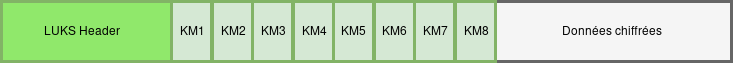
\includegraphics[width=.8\linewidth]{etat_art/format_disque_luks.png}
\caption{\label{fig:LUKSFormat}Format sur disque LUKS}
\end{figure}

\paragraph{}
Les métadonnées de LUKS contenant les algorithmes de chiffrement, 
d'authentification, la version de LUKS, sont suivis de huit emplacements 
permettant de stocker des clés chiffrées, qui permettent de déchiffrer le 
disque. Ainsi on peut stocker la même clé huit fois, protégées par des mots de 
passe différents, permettant ainsi à plusieurs utilisateurs de déchiffrer le 
même disque sans pour autant partager le même mot de passe.

\paragraph{}
Les métadonnées de GELI sont stockées contrairement à LUKS, à la fin du disque.
L'en-tête permet de stocker 2 clés, et s'étend sur un seul secteur.


\paragraph{}
\begin{figure}[h]
\centering
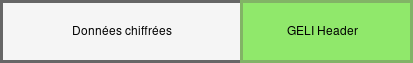
\includegraphics[width=.5\linewidth]{etat_art/format_disque_geli.png}
\caption{\label{fig:LUKSFormat}Format sur disque GELI}
\end{figure}

\paragraph{}
Dans les deux en-têtes on retrouve des champs similaires, un {\em Magic} qui 
permet de connaître le type d'en-tête, la version, l'algorithme de chiffrement 
et d'authentification, etc. On peut noter tout de même que la taille de 
l'en-tête sous GELI fait 255 octets, contre 592 octets pour LUKS.



\subsection{Algorithmes}
\paragraph*{} A rédiger
\subsection{Fonctionnalités}
\paragraph*{} A rédiger
